\chapter[承诺不再丢失：需求与追溯本体]{承诺不再丢失：\\需求与追溯本体}

\begin{noteblock}
Semantica 绑定： 本章保存派生、分配、接口和重开关系的解释；唯一机器语义是
\nolinkurl{semantica.chapter_packages.vol2.ch15}，主场景为
\nolinkurl{semantica.vol2.ch15.scenario.primary}。本体、CQ、查询、Shape、traceability 案例、
规则、oracle、manifest 与 receipt 只在 Semantica。当前为 \nolinkurl{partial}、release
\nolinkurl{blocked}；闭世界检查只在声明范围内成立，不能证明现实依赖已经记全。
\end{noteblock}

\begin{center}
\vspace{0.2em}
\chapterartfade{%
\adjustbox{max size={0.88\linewidth}{0.27\textheight}}{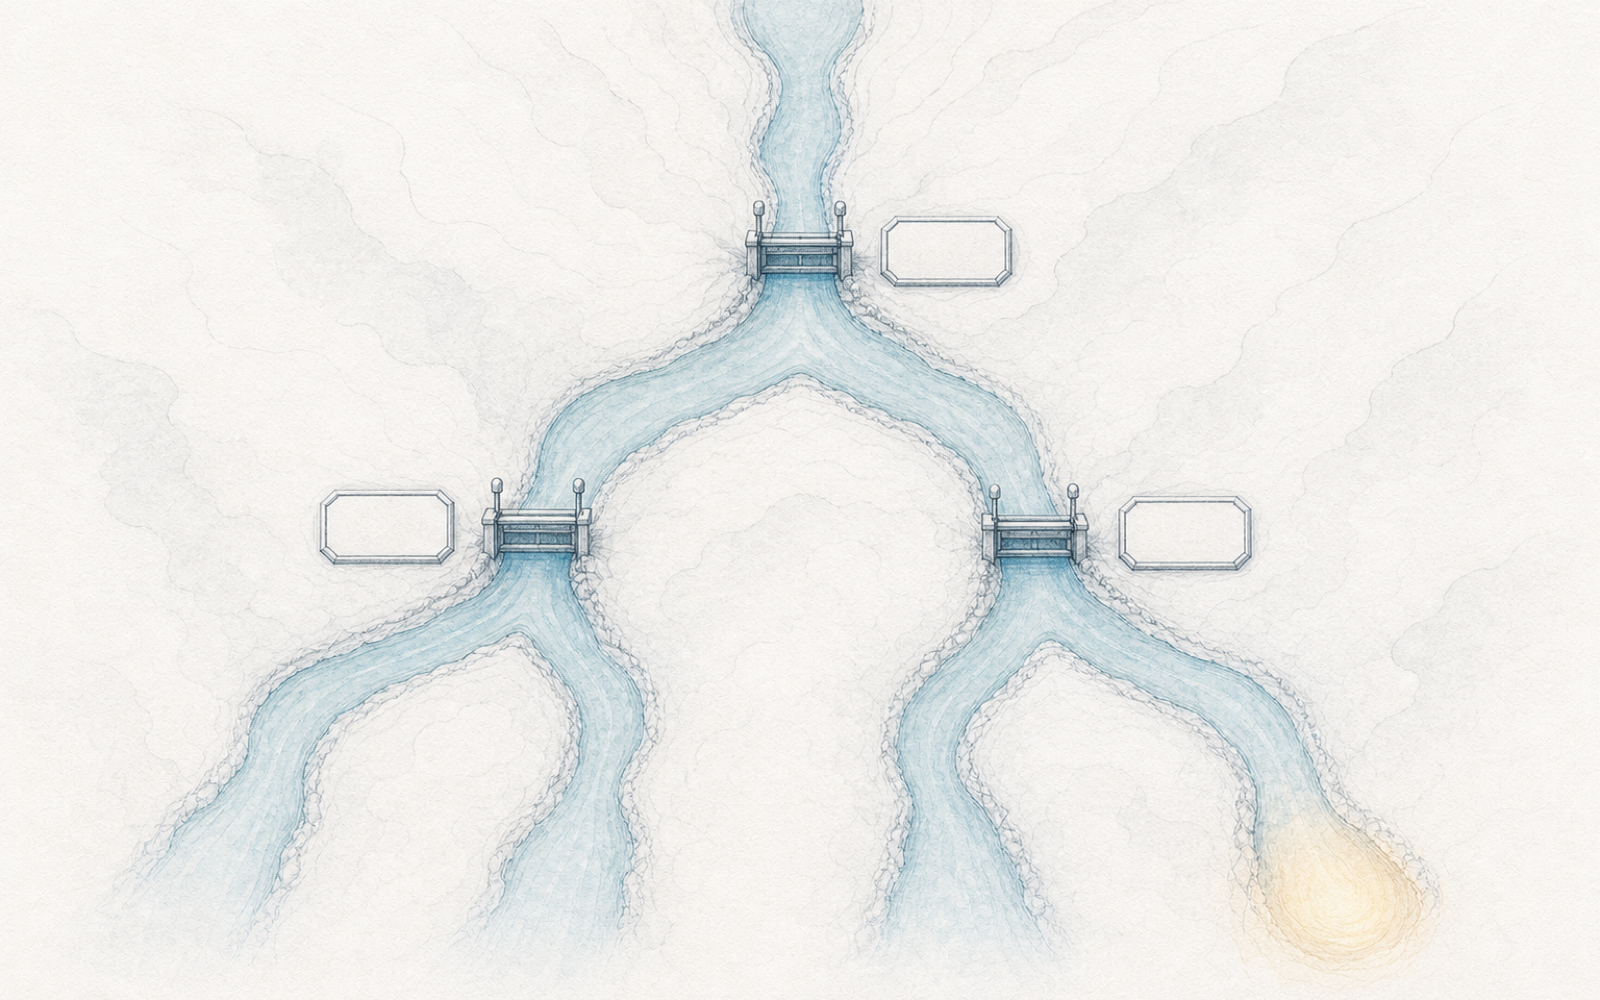
\includegraphics{figures-imagegen/art-ch15-v01.png}}%
}
\vspace{0.35em}
\end{center}

\begin{noteblock}
\textbf{【导读】}
前一章的试点把“担心什么”建成了机器可查的结构，危害定了目标；可目标要落地，
还得流进需求——而系统层那本旧账我们都记得：一场开了两天的会议，一份四十多项、
没有人敢担保完整的重开清单。本章陪小蔡把那本旧账搬进新载体：先看一条需求
怎样从一句话长成一个“缺件即拒”的对象；再看连线怎样被逼着交出理由、分配怎样
被逼着等来确认；然后守在接缝的门口，看当年那个“典型值 2 毫秒”第二次登门时
撞上什么；再给一笔至今待定的时间预算立起账本；最后回答陈工当年那个没人答得动
的问题——“哪些东西要重开”。
读完本章，你应当能把一条需求写成机器可以拒收的对象，并在上游变化的那天，
让机器先于会议室交出重开清单的第一版——同时说得出这份担保的边界画在哪里。
\end{noteblock}

\Needspace{6\baselineskip}
\section{四十多项的清单，翻出来重问}

试点推进到需求这一站的那个早上，小蔡做的第一件事，是把档案里那份清单调了出来：
四十多项，字迹来自好几个人，是当年梁工那封传感器换代邮件之后、整个项目
在会议室里投影矩阵、逐行认领、开了两天才凑出来的东西。散会时没有一个人
敢担保它是完整的——这句记录，就写在清单末尾。她把清单投在试点室的屏幕上，
旁边是团队的 AI 助手的工作区。助手在这个房间里的地位从试点第一天起就没变过：
它提议、它执行，它不是事实的来源，也不是任何事情的决定者。

小蔡自己也不是当年会议室里的旁观者。那两天她刚入职不久，负责给认领结果
做记录，亲眼看着一群她敬重的工程师靠记忆打捞自己半年前的决定。散会时
她在笔记本上写过一行字：“我们不是不认真，我们是没有地方放这些东西。”
现在，地方有了——问题是往里放什么。

安全目标已经在上一站被建成了机器可查的对象，经由显式的对齐合同交到需求世界
门口；本章不重建危害与目标的语义，只在自己的边界内把它们当作上游的锚点。
问题是接下来这一步：目标流进需求的路上，纸面时代丢过三样东西，系统层的
冻结报告写得清清楚楚。其一，追溯靠人手维护，账本永远慢于事实；其二，派生的
理由不留痕，纸面记得住“有关”，记不住“为什么有关”；其三，影响算不出来——
改一条上游，没有任何机械的办法列出下游哪些要重开。

小蔡把这三条翻译成新载体必须回答的问题，写在白板上：

\begin{itemize}
\item 任何时刻指着一条需求问“它完整吗”，机器要能回答缺什么；
\item 任何一条派生连线，机器要能回答“为什么有关、依赖了上游的什么”；
\item 任何一次分配，机器要能回答“接收方确认了没有”；
\item 改一条上游，机器要能交出下游重开清单的第一版，并说清这份清单担保到哪里。
\end{itemize}

陈工看完白板只补了一句：“最后一条，就是我当年问小唐的那句——哪些东西要重开。
这回我想听机器先答。”

要让机器答得动这四问，得先解决一件更基本的事：在机器眼里，
“一条需求”到底得是什么东西？

\Needspace{6\baselineskip}
\section{一条需求，长成一个对象}

纸面时代的需求是一句话，一句话住在表格的一格里。系统层那一章炼出过一条
清点纪律：每一次交接都要重新清点触发、模式、动作、判据、时限，少一样就丢一样。
纪律是对的，丢的方式也早看清了——那句“检出偏差后请求抑制助力”，
拆分之后三个承担者每人领走一个动作，“多快”不在任何一条里。

怎么防？第一反应是把模板做硬：给需求文档加五个必填栏。这一招很多团队试过，
败得很安静——纸面的必填拦得住空白，拦不住敷衍，“时限”一栏里填着“见上文”
“尽快”“待定”的表格，每个项目都能翻出几页。第二反应是设专人复核：每条需求
录入后由资深工程师过一遍。这一招也不算错，但复核也是人手，人手就有周期，
周期就慢于事实；而且复核标准仍在复核人的脑子里，人一换，标准跟着换。

新载体换了一个思路：不把“完整”当成一种事后审查出来的品质，而把它写进
“需求”这个词的定义里。下面这段记法在说什么：它声明了一条技术安全需求，
\Needspace{8\baselineskip}
五个要素各占一行——在这个世界里，五行缺一行，这个对象根本不成立。

\nopagebreak[4]
\begin{codebox}
\begin{Verbatim}[fontsize=\small,breaklines=true,breakanywhere=true,breaksymbolleft={},breaksymbolright={}]
# 一条技术安全需求（示意记法）
req:TSR_TorqueCompare a req:Requirement ;
    req:trigger    "两路转矩信号偏差越过受控阈值" ;    # 触发
    req:mode       req:NormalDriving ;                 # 模式：正常行驶
    req:action     "请求抑制助力并转入降级" ;           # 动作
    req:criterion  "偏差判定与降级进入均可在台架复现" ;  # 判据
    req:timeLimit  req:BudgetItem_Detect .  # 时限：指向账本的一格
\end{Verbatim}
\end{codebox}

注意最后一行：时限不是一个随手填的数，它指向时间账本里的一格——这一格
现在还空着，我们到预算那一节再回来收它。

这个门槛不是跟人过不去。触发说清它盯着什么，模式说清它在系统的哪种状态下
生效，动作说清谁做出什么反应，判据说清拿什么判成败，时限说清多快才算数——
五样合在一起，才是一句别人可以照着做、也可以照着验的承诺；少任何一样，
下游就得靠猜，而猜出来的分歧不会自己暴露，要等台架或者路上才见面。
而且缺哪一样，猜就长在哪一样上：缺时限的下场全书都看过了；缺模式，
抑制逻辑在检修工位上也照样出手，诊断设备刚连上车就被请了出去；缺判据，
开发的人按自己的理解测完说“好了”，验证的人按另一种理解判“不过”，
两份报告都是真的，吵到最后才发现两边验的根本不是同一句承诺。
系统层的正文早把这个道理讲透了，新载体做的只是一件事：把道理变成门。

迁移旧矩阵是 AI 助手的活：它读旧表格，把一行行句子提议成一个个候选对象。
\Needspace{8\baselineskip}
第一批迁移就撞了墙。下面这段示意的是机器怎么拒绝——被拒的正是当年那句话：

\nopagebreak[4]
\begin{codebox}
\begin{Verbatim}[fontsize=\small,breaklines=true,breakanywhere=true,breaksymbolleft={},breaksymbolright={}]
# 机器怎么拒绝（示意）：缺件的句子进不了需求库
输入: "检出偏差后请求抑制助力"        # 从旧矩阵迁来的原句
裁定: 拒收 —— 不构成 req:Requirement
缺件: req:mode（模式）、req:timeLimit（时限）
处置: 降为 req:Memo 暂存，补齐后重新提交
\end{Verbatim}
\end{codebox}

小蔡盯着“缺件”那一行看了很久。当年这个洞，是梁工第一次到场、以一个
局外人的直觉问出来的——“要多快，才算够快？”靠的是运气：恰好有一个
不欠这个项目任何默契的人坐在会议室里。现在同一个洞，是录入的那一秒被
机器指出来的，不需要任何人恰好在场。被拒的句子没有被扔掉，它降级成备忘，
留在暂存区等人补齐——机器拒绝的不是这句话，是它冒充需求的资格。

\textbf{需求的完整性不该是审查出来的品质，而应是存在的门槛：五样凑不齐的句子，可以是备忘，不允许是需求。}

对象立住了。可四十多项清单的病根不在对象上，在对象之间——
那些线，机器怎么知道它们为什么在那里？

\Needspace{6\baselineskip}
\section{连线要带理由，分配要等确认}

迁移进行到第三周，小唐来看图。屏幕上，需求对象一层层挂着，派生连线一条条
校验通过，分配一条不缺。小唐是当年那张全绿矩阵的作者，他看了很久，说：

\textbf{“上次全绿是我手填的表，这次全绿是机器逐条查过的图——每条线都在，每个对象都齐。这回，总算是都接住了吧。”}

这句话比当年那句更不外行。机器校验的图确实严格好于手维护的矩阵：
矩阵记录的是上次有人有空时的世界，图的每一次变更都当场过检；矩阵的格子
可以悬空，图里悬空的对象根本存不进去。如果这样还不算接住，
问题一定藏在校验照不到的地方。

它藏在理由里。评审会上，梁工顺着比对需求的派生线往上看，停住了：
AI 助手迁移时给这条线补的理由写着“比对窗口由上游检出时限派生”——通顺、
体面、结构齐全，校验全绿。可梁工记得真实的历史：当年那个窗口，依据的是
他老款传感器的最坏刷新，跟上游时限没有直接关系。做这个决定的工程师已经
离职，理由不在任何纸面上，助手读不到，就按最像的样子补了一个。
线是真的，理由是编的。

怎么办？第一个提议最省事：让助手把全部理由都生成了，反正它写得又快又通顺。
不行——这正是全书反复立过的界碑：模型的提议不是事实，通顺不是为真，
一条被机器猜出来的理由，比没有理由更危险，因为它长得像证据。第二个提议
是把校验规则加严：理由不许是一段散文，必须指认“依赖了上游的哪个具体部分”。
这一条被采纳了——有了锚点，理由第一次变得可以被证伪；但采纳之后大家发现
它仍然不够：锚点保证理由可查，保证不了理由为真。为真只有一条来路：
一次有记录的确认活动——评审、会签，或者像梁工这样当场指认历史。

于是这条线被打回“提议”状态，走了一整圈才重新变绿。这一圈值得慢放，
因为它就是助手在这个世界里被允许的全部动作：第一步，提议——助手根据
旧矩阵和会议纪要给出连线和理由的候选，候选带着明显的记号，任何查询都不会
把它当成事实取走；第二步，校验——机器查结构，五要素、锚点、出处，
缺一样打回；第三步，确认——梁工在评审里给出真实依据，小唐署名确认，
这一步只能由人完成，候选从这一刻起才是事实；第四步，审计——谁提议、
谁改写、谁确认、发生在哪一天，全程留痕，半年后有人再问“这条线谁认的”，
不需要任何人的记忆在场。那条编造理由的线，正是在第三步被拦下的——
前两步机器全绿，恰好证明了机器的绿灯照不到“为真”。

下面这段记法在说什么：它是那条改正之后的连线——理由不再是
\Needspace{8\baselineskip}
一段话，而是一个对象，带着锚点、说法和出处。

\nopagebreak[4]
\begin{codebox}
\begin{Verbatim}[fontsize=\small,breaklines=true,breakanywhere=true,breaksymbolleft={},breaksymbolright={}]
# 一条带理由的派生连线（示意记法）
req:Der_042 a req:Derivation ;
    req:fromReq  req:FSR_DetectAndMitigate ;      # 上游：功能层承诺
    req:toReq    req:TSR_TorqueCompare ;          # 下游：比对需求
    req:rationale [ a req:DerivationRationale ;
        req:dependsOnAspect req:Param_SensorUpdate ;  # 锚点：传感器更新特性特性
        req:justification   "比对窗口按老款传感器最坏刷新设定" ;
        req:confirmedIn     req:ReviewRecord_P15_03 ] .  # 出处：本次评审记录
\end{Verbatim}
\end{codebox}

锚点那一行请记住——它指向的不是一条需求，而是接缝上的一个参数。
这个细节要到本章最后一节才显出它的分量。

分配也是同一个道理。旧矩阵里“每条需求都有主儿”，可没有一处记录着
主儿点过头——认领发生在邮件里、走廊上、周会的口头应答里，等到要追问
“这条你当时是怎么理解的”，对话早已蒸发。新载体里，一次分配在接收方
确认之前一直处于“悬空”状态，悬空不是错误，但它挂在图上人人可见，
且不允许被任何下游结论引用；确认也不是点一下按钮，接收方确认的内容
被写明了——确认的是这条需求的五要素在我的边界内可实现、可验证，
基于此刻图里记录的接缝参数和预算格子。基于什么而确认，日后就凭什么
而重开。
到这里，三样东西第一次在情节里站成了三角：本体规定什么算一条成立的
连线——这是语义；连线为真，来自评审与会签这些受控活动——这是事实；
而当两个团队对“当年依据”各执一词时，拍板的仍然是有权的人——那天下午
有一条争议线,最后是陈工裁的。三样各归各位，谁也替不了谁。

\textbf{连线证明的是存在，不是成立；一条派生要成立，得说得出依赖了上游的什么——而“为真”永远来自确认它的活动，不来自画出它的手。}

这条界线值得追问一层：为什么一代又一代的组织，都心甘情愿把“全绿”
当成“接住”？因为存在查起来便宜，成立查起来贵。线在不在，外人扫一眼
就能数完；理由真不真，得把当年的历史请回来才问得动。于是评审对着
看得见的连线提问，审核对着留了痕的步骤抽查，考核给数得出来的完整率
发奖——三股压力全都压在“形”上，没有一股压得到“义”。一条编得通顺的
理由在这种环境里不但活得下去，还活得最好：它喂饱了每一次检查，
把唯一拆得穿它的那个人——记得真实依据的人——留给运气。全绿不是谎言，
它只是把没人查得动的那部分，藏进了绿色里。

线也立住了。可小蔡心里还悬着一件事：当年最疼的那一跤，
不是摔在需求上，是摔在接缝上——那个 2 毫秒，换了载体还会不会重演？


\begin{noteblock}
\textbf{读图任务}：跟随左右节点之间的每条连线，检查线中间的理由牌是否存在，再找到一条理由缺失和一条末端搭扣尚未闭合的关系。
\end{noteblock}

\begin{center}
\begin{minipage}{\linewidth}
\centering
\adjustbox{max size={\linewidth}{0.78\textheight}}{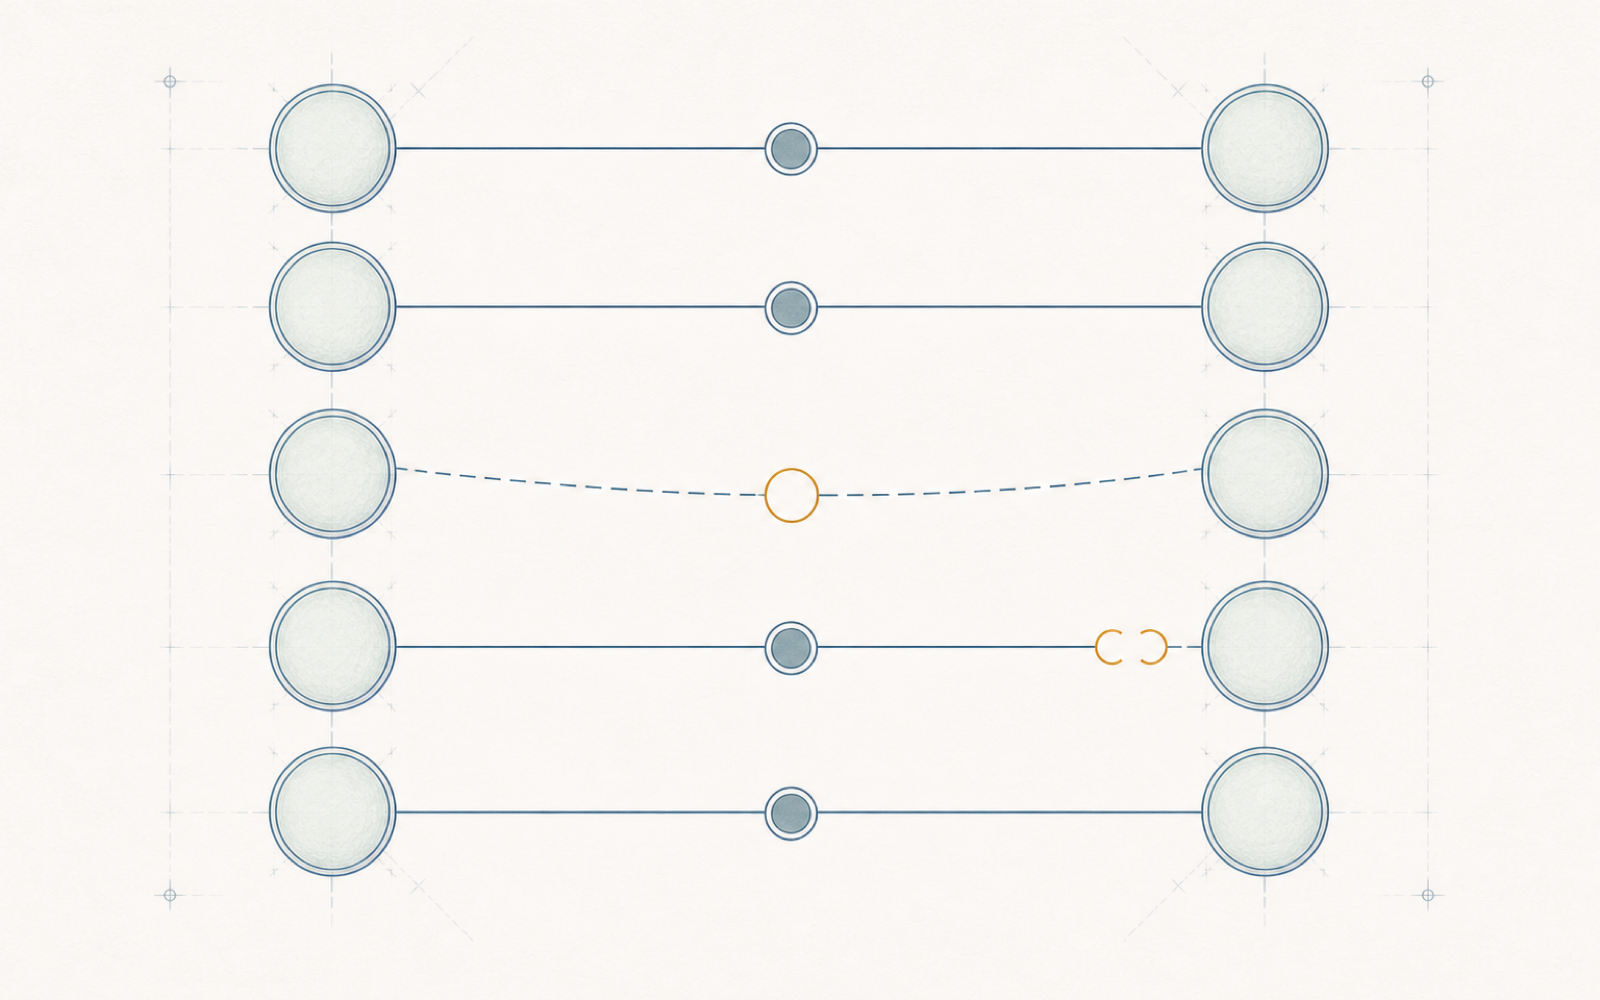
\includegraphics{figures-imagegen/ch15-fig01-reasoned-allocation-v01.png}}
\captionof{figure}{需求追溯不是两个 ID 之间的裸连线。每一次派生、分解、分配或满足都要交代理由，而分配边在承接方确认前仍然是待定状态。}
\end{minipage}
\end{center}


\begin{noteblock}
\textbf{图后判断}：本图不会因连线完整就证明需求正确，也不代替技术实现、验证或组织授权。理由对象自身仍需可追溯事实支持。
\end{noteblock}

\Needspace{6\baselineskip}
\section{两毫秒，第二次来到门口}

低温台架那三天，这个项目的老人都记得：手册是真的，表是认真填的，代码是
照表写的，助力还是时断时续。病根事后看得清清楚楚——接口表誊抄时留下了
“2”，丢掉了“典型”两个字和那行低温条件；事后的补救也做得不可谓不重，
两百多行逐行补了“条件”和“最坏值”两列，重新会签。

可小蔡把当年的补救翻出来看，越看越不安：补上的是那张表，不是抄表这件事。
只要接缝上的数字还靠人从文档往表里搬，“典型值”三个字就总有一天会再次
被搬丢。有人说，加强培训，录入前先读脚注——可当年那张表恰恰是逐行核对
过的，认真拦不住结构性的洞。有人说，把供应商手册整册挂进系统，随时可查——
可见不等于承诺，这个坑当年就排除过一次：手册是对器件的描述，不是对
这个项目的担保，挂得再近，脚注照样可以被路过。

新载体的做法，是把当年补进表里的那两列，升格为接缝参数这个对象的
构成条件。试点里立的规矩：接缝上的每一个数字，必须以参数对象的身份入库，
值、成立条件、最坏值、最坏值出现的条件、坏了怎么说、谁承诺——缺一个字段，
这个数进不了门。

重演的那一幕发生在一个很平常的下午。一位新来的工程师把老接口合同往
载体里迁，敲到传感器那一行，顺手录入：“更新周期，2 毫秒。”回车。
机器拒收：缺“成立条件”，缺“最坏值”。他愣了一下，回头去翻合同，
把补签过的那两列找出来，重新录入，这次过了。前后不到十分钟，
没有台架，没有零下三十度，没有五周的重新排队。

消息传到软件组，小林特意走过来看了一眼屏幕。当年说出“接口表都填满了，
两边照表干活就行”的人是她，低温里查了三天自家滤波和去抖的人也是她。
她看完那条拒收记录，只说了一句：“当年要是有这道门，我那三天就不用查了——
门口就断案了。”梁工看完那条拒收记录，说了一句话，后来被小蔡记进了试点日志：
“我在手册里写了十五年脚注，今天第一次看到一个系统规定脚注不许被抄丢。”
下面这段记法在说什么：它是那条最终入库的参数——当年脚注里的
\Needspace{8\baselineskip}
每一样东西，现在都是必填字段。

\nopagebreak[4]
\begin{codebox}
\begin{Verbatim}[fontsize=\small,breaklines=true,breakanywhere=true,breaksymbolleft={},breaksymbolright={}]
# 接缝上的一个参数：值、条件、最坏值缺一不可（示意记法）
req:Param_SensorUpdate a req:InterfaceParam ;
    req:typicalValue "2 ms" ;
    req:validUnder   "常温、低温补偿未激活" ;    # 典型值何时成立
    req:worstCase    "8 ms" ;                    # 最坏值（合成示例数字）
    req:worstUnder   "低温补偿运行" ;             # 最坏值出现的条件
    req:failureTell  "更新停滞时诊断位按时置位" ;  # 坏了怎么说
    req:committedBy  req:SupplierCommit_L07 .    # 谁对本项目承诺
\end{Verbatim}
\end{codebox}

最后一行同样是承诺换手的记录：这个 8 毫秒不是从手册里抄来的描述，
而是供应商对这个项目的承诺，有出处、有署名。手册的脚注当年只说
“最坏可达数倍”——“数倍”是写给所有客户的措辞，没法拿来设计窗口；
8 毫秒是供应商第一次把“数倍”对这个项目钉成一个可以按计算器的数：
四倍于典型值，签了名。软件的比对窗口从此对着
最坏值那一格设计，而不是对着典型值。

\textbf{一个不带条件的数字，在接缝上不是信息，是伏笔；载体的职责是让“典型值”三个字无处藏身——要么把条件和最坏值一并交出，要么这个数进不了门。}

数字进了字段，新的问题跟着来了：8 毫秒也好，置位时限也好，读走窗口也好，
这些毫秒最终都要从同一笔总账里扣。可这套系统的总账——那个容忍窗口——
到今天还写着“待定”。待定的账，怎么记？

\Needspace{6\baselineskip}
\section{待定的窗口，也要有账本}

从故障出现到危害可能形成的那个窗口，属于危害和整车情境，不属于任何机制——
这条纪律是系统层用一个下午的评审换来的，试点原样继承。而这个窗口的数值，
从概念阶段冻结到今天，一直是“待定”：车辆动力学分析还在进行，数字要靠
分析和试验去挣，不能先抄一个好看的整数。

待定的窗口怎么进载体？第一个提议：先填一个保守的占位值，标注“临时”，
免得账本空着难看。不行——这是全书埋葬过不止一次的做法：没有来源的数字
一旦进了系统，就会被下游当真，“临时”两个字的下场和“典型”两个字不会有
任何不同。第二个提议：那就等窗口定了值再建账。也不行——系统层的教训
原文还在：等数字来了再立账本，各段时延早已各自为政。

新载体给出的第三条路，是把“待定”本身建成一个受控状态。下面这段记法
在说什么：它是那笔预算的账本——窗口一格明确记为待定，待定有主人、
有在办的活动；各段的最坏值凡是有承诺的，逐格入账；而余量一格，
\Needspace{8\baselineskip}
记的既不是零，也不是某个数，而是“未知”。

\nopagebreak[4]
\begin{codebox}
\begin{Verbatim}[fontsize=\small,breaklines=true,breakanywhere=true,breaksymbolleft={},breaksymbolright={}]
# 一笔待定的预算（示意记法）
req:LedgerFaultToSafe a req:TimeBudget ;
    req:totalWindow  req:Pending ;              # 容忍窗口：待定
    req:pendingOwner "车辆动力学分析（进行中）" ;  # 待定有主，不是没人管
    req:hasItem req:BudgetItem_Sense ,  # 传感段：最坏 8 ms（接缝承诺）
                req:BudgetItem_Detect ,         # 检出一段：最坏值已承诺
                req:BudgetItem_React ;          # 反应一段：最坏值已承诺
    req:margin  req:Unknown .                   # 余量：未知（非零也非够）
\end{Verbatim}
\end{codebox}

这本账立起来之后，机器多了一种从前没有的诚实。有人在评审里问“现在余量
够不够”，机器的回答是：各段已承诺的最坏值合计若干毫秒，窗口待定，
余量未知，不予判定。它拒绝说“够”，也拒绝说“不够”——未知就是未知，
这是从术语那一章一路继承下来的三值纪律。而它同时承诺了一件事：窗口定值
的那一天，余量自动重算，凡是引用过这本账的结论逐条标示重查。上一节
那条比对需求的时限，指的就是这本账里的一格——格子先画好，数字到位那天
才有处可记，这句话现在是机器行为，不再是口号。

陈工对这一格的评价只有一句：“以前‘待定’写在表里，是等着被人忘掉的；
现在它写在账上，是等着来讨债的。”讨债的日子不归机器定——分析何时收口、
数字何时算挣到了手，仍然由做分析的人和有权接受它的人说了算；
账本只保证：那一天来的时候，没有一个依赖它的格子能装作没听见。

\textbf{待定不是空白，是一种受控状态：它有名字、有主人、有到期的义务，并且向下传染——凡是依赖它的结论，一律不得早熟。}

五要素、理由、确认、条件、账本，都立住了。那么，现在可以回答
陈工那个问题了：改一条上游，哪些东西要重开？

\Needspace{6\baselineskip}
\section{重开清单，这一次机器先说}

机会来得比预想快。传感器换代的第二波通知到了：新款的设计资料包发放，
老款停产进入倒计时——当年引发两天会议的那场变更，现在真的落地了。
换代意味着一件确定的事：老款传感器的最坏刷新承诺，将随老款一起失效。

小蔡没有订会议室。她让助手对着载体提了一个问题。下面这段是问题、
查询和答案的三段式——查询做的事说穿了很朴素：把所有理由里引用了
那个传感器参数的连线，连同它们指向的下游，一次取出来。

\Needspace{8\baselineskip}
问题：传感器换代，最坏刷新承诺失效——下游哪些对象的成立理由引用了它？

\nopagebreak[4]
\begin{codebox}
\begin{Verbatim}[fontsize=\small,breaklines=true,breakanywhere=true,breaksymbolleft={},breaksymbolright={}]
SELECT ?affected ?why
WHERE {
  ?edge  req:rationale       ?r .
  ?r     req:dependsOnAspect req:Param_SensorUpdate .  # 理由锚在这个参数上
  ?edge  req:toReq           ?affected .
  ?r     req:justification   ?why .
}
\end{Verbatim}
\end{codebox}

答案（节选）：

\begin{center}
\begingroup\small
\setlength{\tabcolsep}{4pt}
\begin{tabularx}{\linewidth}{@{}XXX@{}}
\toprule
受影响对象 & 为什么有关 & 建议动作 \\
\midrule
比对需求（TSR\_\allowbreak{}TorqueCompare） & 比对窗口按老款最坏刷新设定 & 重开派生评审 \\
预算条目（BudgetItem\_\allowbreak{}Sense） & 传感段最坏值出自该承诺 & 重新取值入账 \\
接缝合同相关条目 & 置位与读走窗口以该参数为前提 & 重签确认 \\
软件侧的一次分配 & 接收确认基于旧最坏值 & 重新确认 \\
若干验证结论 & 判据引用旧参数 & 重新验证 \\
\bottomrule
\end{tabularx}
\endgroup
\end{center}

查询跑完不到一分钟。小蔡把结果和当年那份四十多项的清单并排放着看：
当年两天会议凑出来的东西，很多行在这里，是被理由锚点逐条钓出来的；
当年清单上没有、这里却有的，是那几条“悬空的分配”——旧世界根本没有
地方记录“确认基于什么”，所以连丢都丢得无声无息。还有一行让小唐
在屏幕前站了很久：比对需求赫然在列，理由一栏写着“比对窗口按老款
最坏刷新设定”——当年做这个决定的人已经离职，两天会议里这条依赖
是靠半张旧会议纪要碰运气碰出来的；这一次，它是被那条改正过的连线
自己交出来的。理由被留下的那一天，没人知道它会在哪一天救场；
它只是等在那里。

系统层的结尾曾请读者做过一件练习：假装收到一封换型邮件，手工列出
重开清单，给自己计时，然后问敢不敢担保没漏——并记住那种不踏实。
此刻可以对照了：不踏实没有被勇气治好，它是被换掉了载体。

但小蔡没有让庆祝发生。她当着陈工的面把丑话说完：这份清单担保的
范围有边界。有人提议把担保做大——让机器把“可能相关”的也全列上，
宁滥勿缺；不行，无差别的“可能相关”会把清单撑回四十多项的规模，
两天会议换个形式重开。有人提议再用人工圈一遍补漏；也不对症，
那等于承认机器清单不可信，回到记忆与运气。真正的答案是把担保
说精确：需求、派生、分配、接缝、预算这几类依赖，试点已经做过
“记录完整”的显式声明，声明范围之内，机器担保一网打尽——凡记了
理由的依赖，一条不漏；声明范围之外——比如试验资产与证据侧的
牵连——机器不担保，清单末尾自动附注了这一句。清单本身也只是提议：
每一行的“重开”要不要立项、何时立项，签字的是陈工，不是查询。

\textbf{机器能担保的是账本之内的一网打尽；人的担保从此换了对象——不再担保“没有漏掉的下游”，而是担保“没有漏记的依赖”。这不是把责任推给机器，是把责任放到人担得动的地方。}

散会前陈工问了最后一个问题：“当年我问‘哪些要重开’，没人答得动；
今天机器答了。那清单最后一列呢——那些‘重新验证’，拿什么算验完？”

\Needspace{6\baselineskip}
\section{清单的最后一列}

小蔡顺着清单往下看。“重开派生评审”，载体里有位置；“重新取值入账”，
账本的格子等着；“重签确认”，确认活动有记录可留。可“重新验证”这一列，
需求世界给不出答案——验证要拿数字作证：一个实测的更新周期、一个实测的
置位时延、一条判据边上的实测裕量。而数字这种东西，本书前半部分用一整章
的硬件教训证明过：脱离对象、方法、条件和来源的数字，不是证据。

需求本体能做的，是把判据和时限写成机器可查的承诺；承诺兑现与否，
要靠带着出处的测量结果来回答——那是另一个世界的事，需要它自己的对象、
自己的门禁、自己的诚实边界。经由显式的对齐合同，这份“重新验证”清单
将交到那个世界门口。

导读的期票，现在兑现：你已经看过一条需求怎样因为缺件被拒收，一条连线
怎样被逼着交出理由，一个“典型值”怎样在门口被拦下，一笔待定的预算
怎样诚实地记账，以及一份重开清单怎样在一分钟内替代两天会议——连同
它担保的边界。承诺不再丢失，靠的不是更认真的人，而是一个丢了就
存不进去的载体。

下一章的问题，梁工在离开评审室时替所有人问了出来：
“重新验证的时候，我给你的每一个数——你们拿什么记住它是在哪儿、
怎么量出来的？”


\begin{noteblock}
\textbf{本章注记}：本章的人物、会议、事故经过与全部数字（更新周期、最坏值、
迁移批次、清单行数、用时等）均为合成教学材料，不对应任何真实企业、
真实产品或真实个人；文中“8 毫秒”等数值仅为教学示例，不是任何实际系统
的参数；容忍时间窗口在本章保持“待定”语义，不构成任何取值建议。
正文对功能安全标准内容的转述为自然语言概括，精确表述以标准原文为准。
各记法片段是有意简化的教学投影；唯一可执行版本是
\nolinkurl{semantica.chapter_packages.vol2.ch15}，当前为 \nolinkurl{partial}、release \nolinkurl{blocked}。
\end{noteblock}
